\begin{frame}{Принципиальные ограничения}
    На основании анализа алгоритма Nanite выявлены следующие принципиальные ограничения, для преодоления которых потребуется разработка новых алгоритмов:
    \begin{itemize}
        \item Оценка искажения не зависит от направления взгляда
        --- иногда разрешение монитора позволяет сэкономить, но определить это нельзя
        \item Невозможность анимации меша --- будет нарушено свойство графа, и его нельзя быстро восстановить
        \item Невозможность автоматической децимации некоторых мешей, напр. листвы --- технология к таким мешам неприменима
        \item Необходимость использовать меши сверхвысокого разрешения, иначе переключения лодов сильно заметны
    \end{itemize}
\end{frame}

% \begin{frame}{Принципиальное ограничение: объём}
%     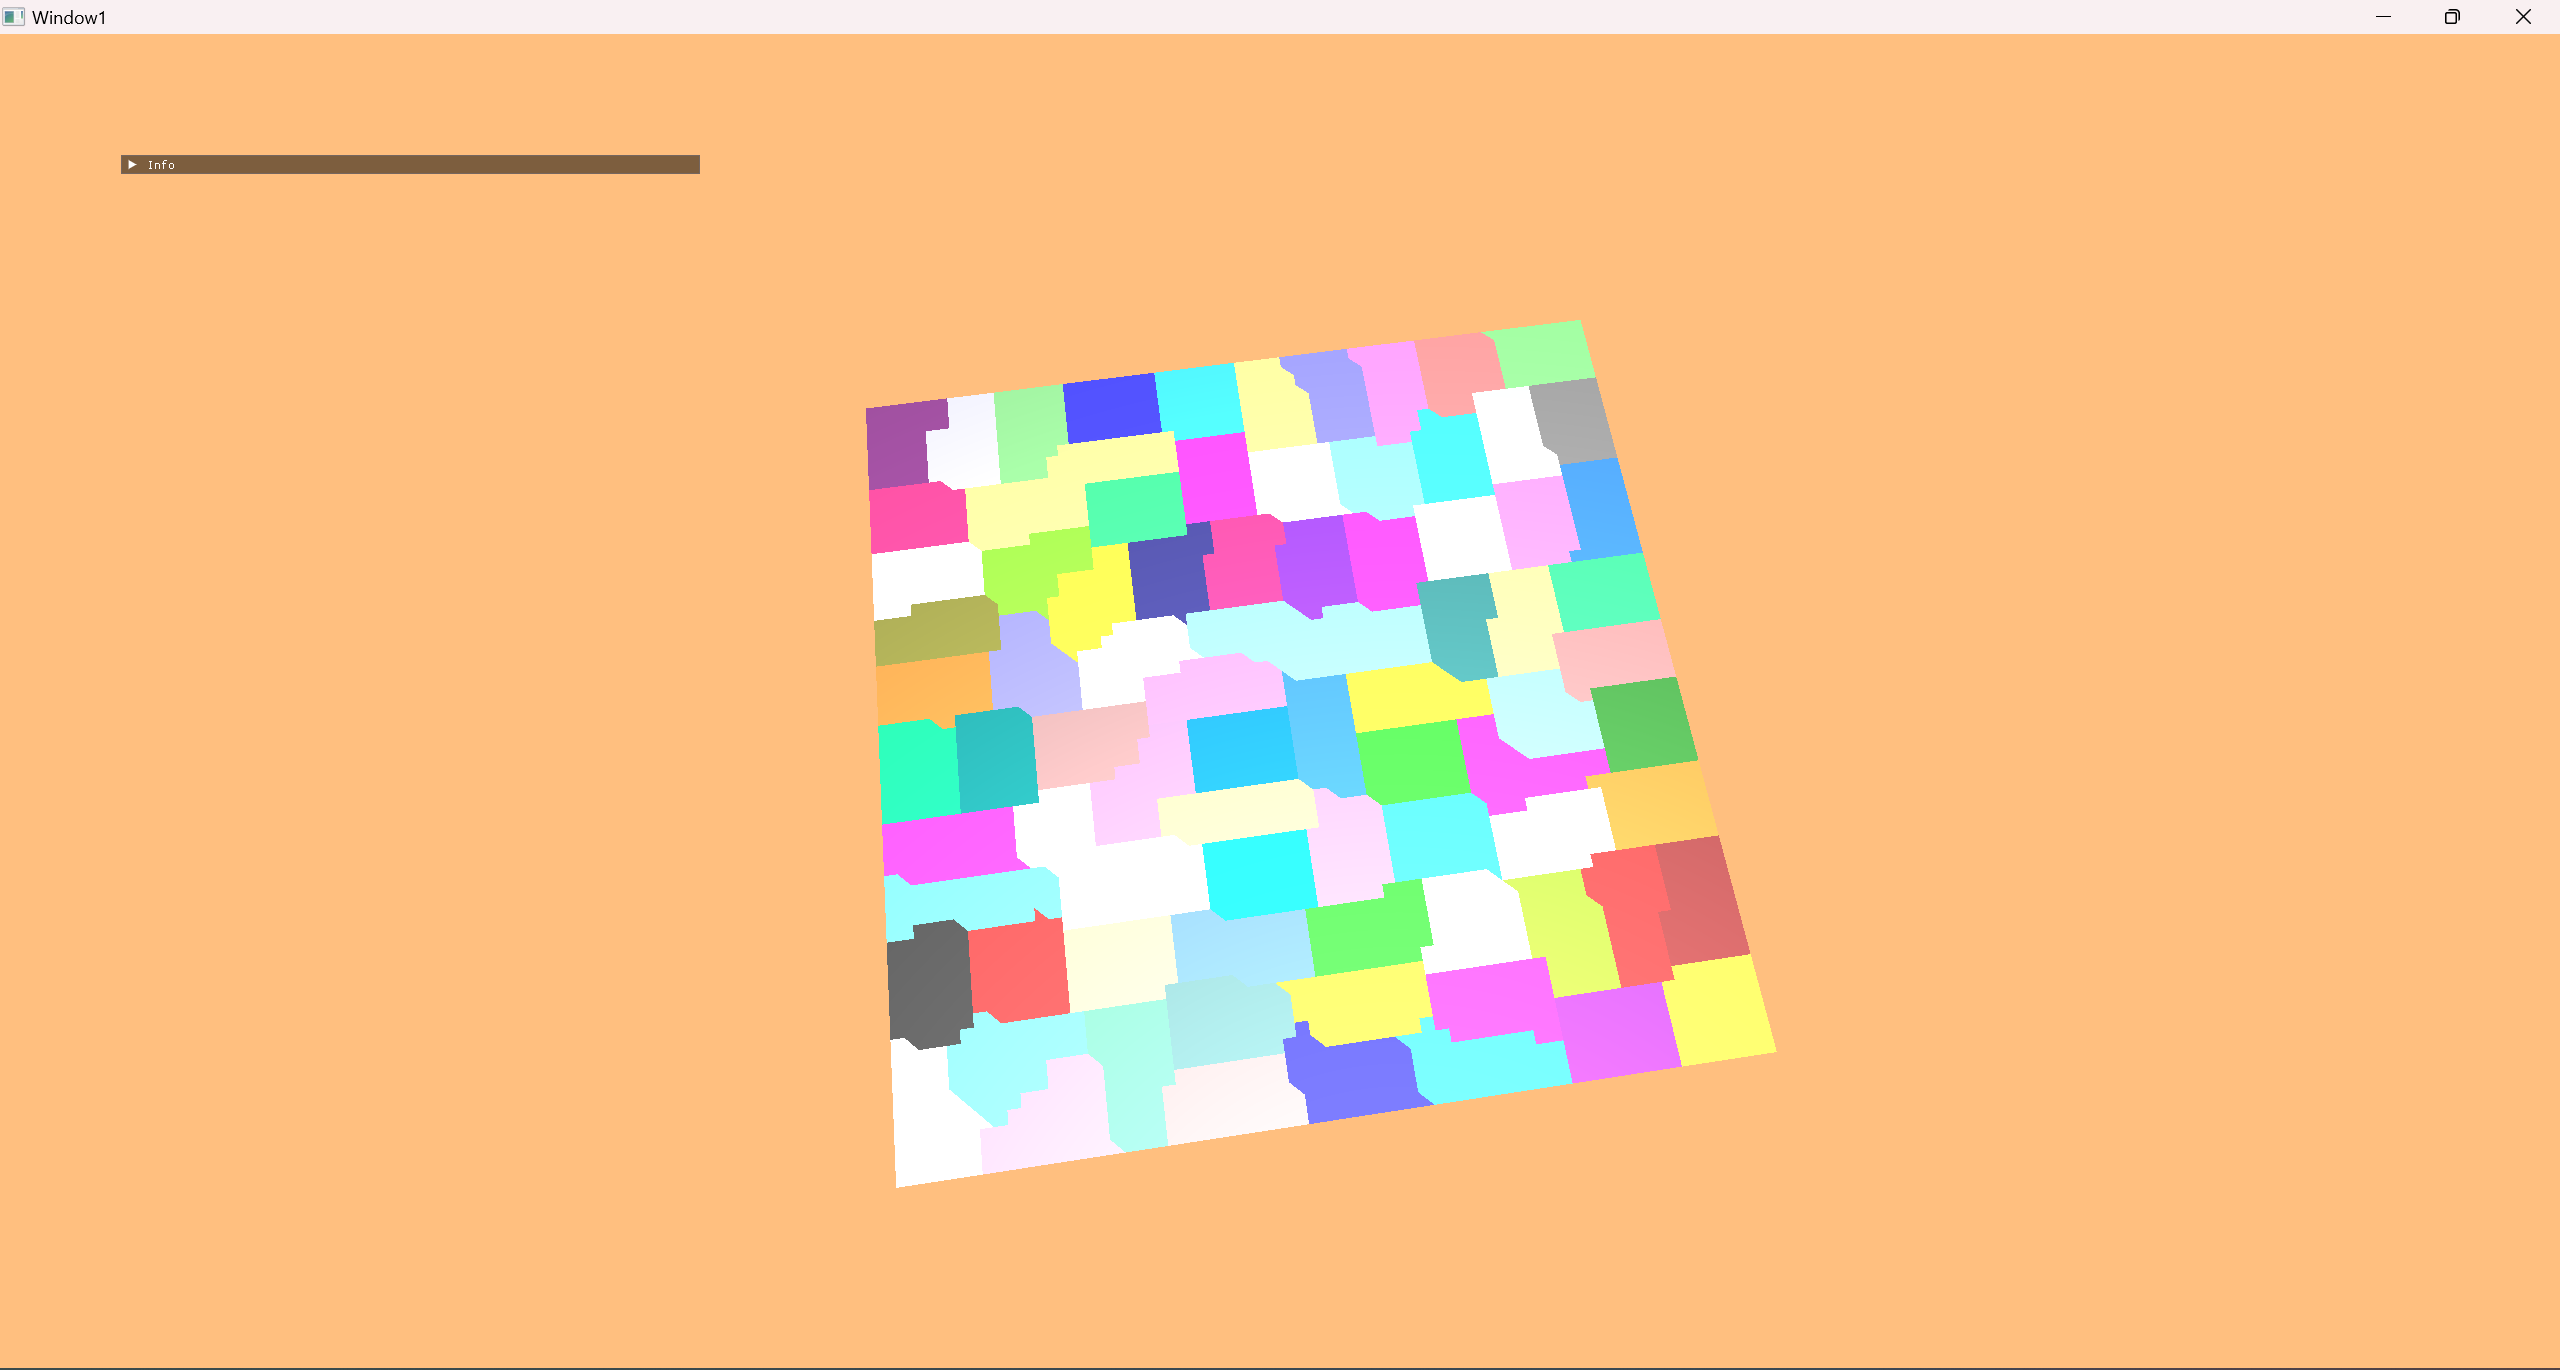
\includegraphics[width=\textwidth]{plane0.png}
% \end{frame}

% \begin{frame}{Принципиальное ограничение: объём}
%     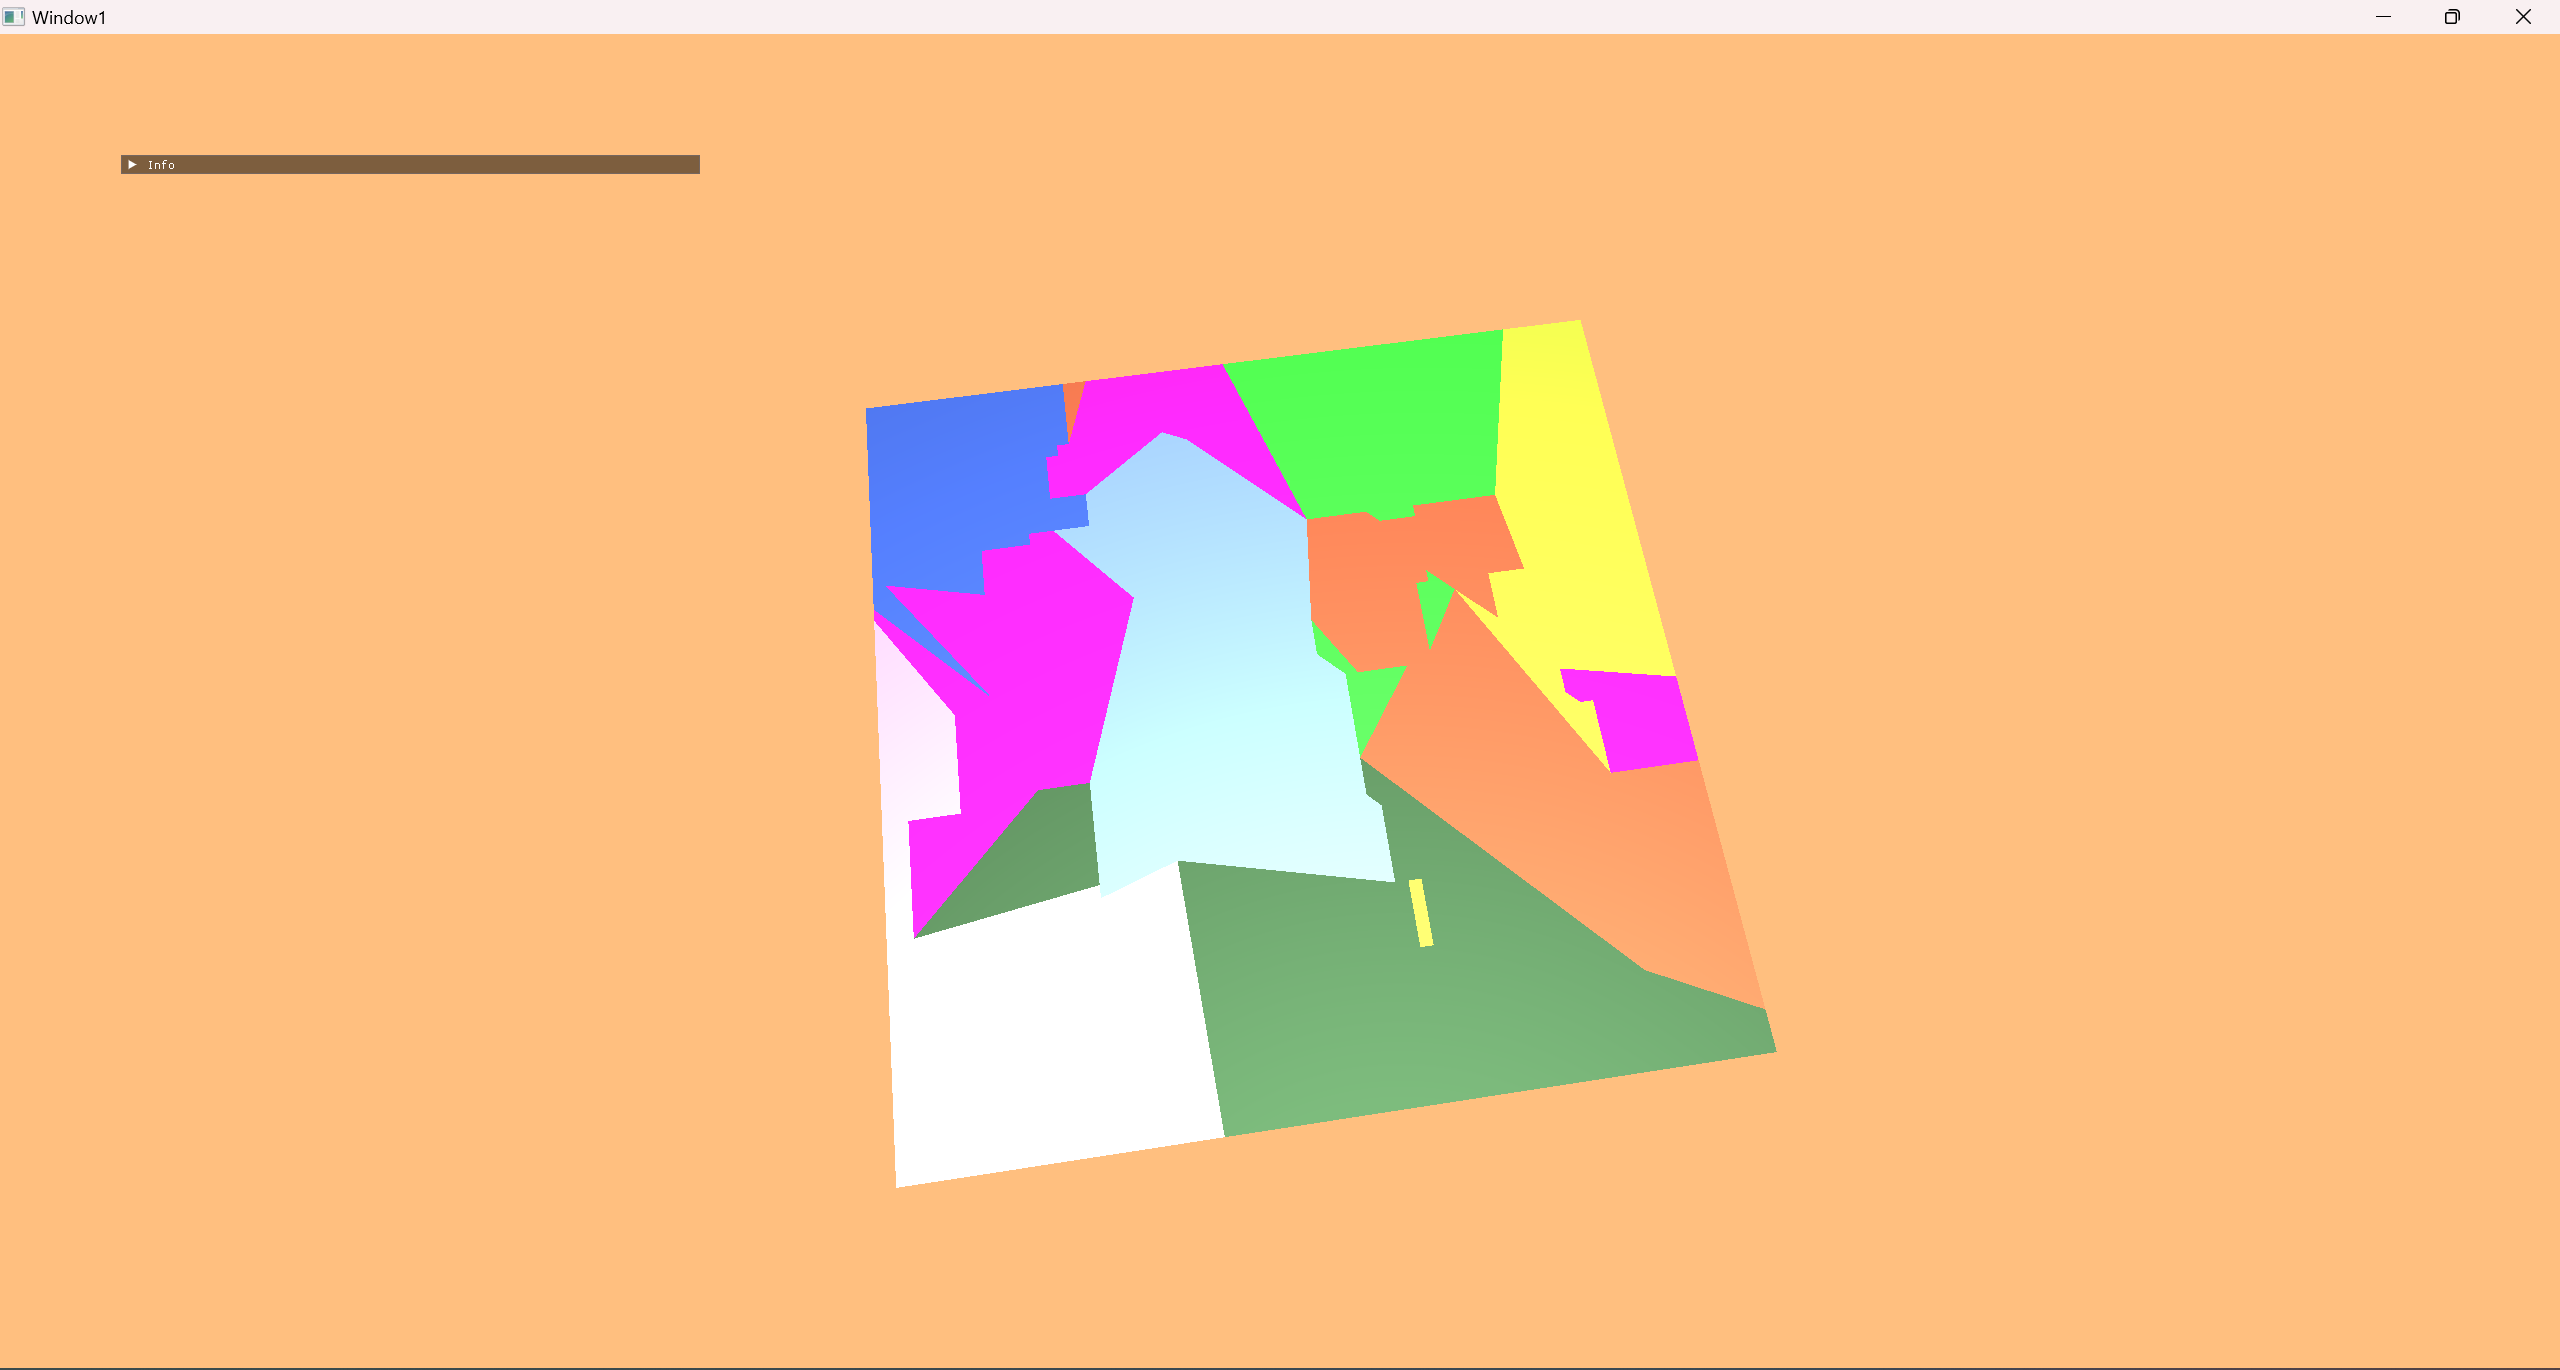
\includegraphics[width=\textwidth]{plane1.png}
% \end{frame}
